\documentclass{article}
\pdfpagewidth=8.5in
\pdfpageheight=11in
\usepackage{ijcai21}
\usepackage{times}
\usepackage{soul}
\usepackage{url}
\usepackage[hidelinks]{hyperref}
\usepackage[utf8]{inputenc}
\usepackage[small]{caption}
\usepackage{graphicx}
\usepackage{amsmath}
\usepackage{amsthm}
\usepackage{booktabs}
\usepackage{algorithm}
\usepackage{algorithmic}
\urlstyle{same}

\usepackage{cleveref}
\crefname{figure}{figure}{figures}
\Crefname{figure}{Figure}{Figures}

\usepackage{tikz}
\usetikzlibrary{shapes}

\newtheorem{proposition}{Proposition}
\newtheorem{corollary}{Corollary}

\newcommand{\citet}[1]{\citeauthor{#1} \shortcite{#1}}

\usepackage{complexity}

\pdfinfo{
/TemplateVersion (IJCAI.2021.0)
}

\title{Solving Graph Homomorphism and Subgraph Isomorphism Problems Faster Through Clique Neighbourhood Constraints}

\author{
Sonja Kraiczy$^1$
\and
Ciaran McCreesh$^2$
\affiliations
$^1$University of Oxford\\
$^2$University of Glasgow\\
\emails
ciaran.mccreesh@glasgow.ac.uk
}

\newcommand{\neighbourhood}{\operatorname{N}}
\newcommand{\vertexset}{\operatorname{V}}
\newcommand{\degree}{\operatorname{deg}}
\newcommand{\nds}{\operatorname{S}}

\begin{document}

\maketitle

\begin{abstract}
    Graph homomorphism problems involve finding adjacency-preserving mappings between two given
    graphs.  Although theoretically hard, these problems can often be solved in practice
    using constraint programming algorithms. We show how techniques from the state-of-the-art in
    subgraph isomorphism solving can be applied to broader graph homomorphism problems, and
    introduce a new form of filtering based upon clique-finding. We demonstrate empirically that
    this filtering is effective for the locally injective graph homomorphism and subgraph
    isomorphism problems, and gives the first practical constraint programming approach to
    finding general graph homomorphisms.
\end{abstract}

\section{Introduction}

The \emph{subgraph isomorphism problem}, as defined by \citet{DBLP:books/fm/GareyJ79}, is to
determine whether an injective mapping exists from one given graph to another, such that adjacent
pairs of vertices are mapped to adjacent pairs of vertices, and non-adjacent vertices are mapped to
non-adjacent vertices.  However, in application-oriented papers, particularly from bioinformatics
and chemistry, the same name is often implicitly used to mean the \emph{non-induced} version of the
problem (which does not require that non-adjacency be preserved) since this more accurately models
the real-world problem being solved \cite{Willett1999,EhrlichR11}. Despite being theoretically hard
problems, these applications, along with others in areas including compilers
\cite{DBLP:conf/cp/BlindellLCS15}, graph databases \cite{DBLP:journals/jair/McCreeshPST18} and
pattern recognition \cite{DBLP:journals/ijprai/FoggiaPV14}, have given rise to a large amount of
research into designing practical algorithms for solving these problems.  Most approaches are based
either upon very fast but simple backtracking algorithms
\cite{DBLP:journals/pami/CordellaFSV04,DBLP:journals/bmcbi/BonniciGPSF13,DBLP:conf/gbrpr/CarlettiFSV17}
which often but not always perform well on very easy instances, or upon constraint programming
algorithms
\cite{DBLP:journals/constraints/ZampelliDS10,DBLP:journals/ai/Solnon10,DBLP:conf/cp/AudemardLMGP14,DBLP:conf/cp/McCreeshP15,DBLP:conf/cpaior/ArchibaldDHMP019},
which have higher startup costs but that perform vastly better on harder instances and much more
consistently on easy instances \cite{DBLP:journals/jair/McCreeshPST18,DBLP:conf/gbrpr/Solnon19}.

The current state of the art is the Glasgow Subgraph Solver \cite{DBLP:conf/gg/McCreeshP020}, which
is a dedicated constraint programming solver for subgraph-finding problems. Much of its performance
comes from inference strategies based upon degrees and neighbourhood degree sequences
\cite{DBLP:journals/constraints/ZampelliDS10}, counting paths between vertices
\cite{DBLP:conf/cp/AudemardLMGP14,DBLP:conf/cp/McCreeshP15}, and cardinality reasoning
\cite{DBLP:journals/ai/Solnon10}, which can be used to eliminate many infeasible candidate
assignments without search. Like most other solvers, it can handle both the non-induced version of
the problem and the traditional induced variant, and users can select whichever variant
better fits their application. It also supports directed edges, and can use an external constraint
solver to handle other extensions to the basic notion of a graph, such as temporal networks and
multi-graphs.

As well as questions over exactly how edges are represented and mapped, some applications would
prefer not to specify injectivity. A \emph{graph homomorphism} is a function between two graphs that
maps adjacent vertices to adjacent vertices, with no injectivity requirement, whilst a \emph{locally
injective homomorphism} is one which is injective when restricted to any individual vertex and its
neighbourhood. Both are better models for some applications
\cite{DBLP:journals/dam/FialaKK01,DBLP:conf/semweb/Baget05,DBLP:conf/iccs/CorbyF07,DBLP:journals/csr/FialaK08,DBLP:journals/pvldb/FanLMWW10,DBLP:journals/tcs/ChaplickFHPT15}.

These injectivity relaxations have received much less attention
from a practical solving perspective.  One might hope that the inference techniques developed for
subgraph isomorphism would also be helpful for other graph homomorphism problem variants. Indeed,
this paper proves that many, but not all, of these strategies are also valid in the locally
injective case, and that simple distance filtering is valid for all homomorphisms.  However, we also
show that \emph{none} of the other strategies are valid for finding homomorphisms where there is no
injectivity requirement.  Finally, we introduce a new filtering technique that is based upon finding
a maximum clique in the neighbourhood of each domain vertex, which is valid even in the general
case. Although this new filtering technique involves solving many additional \NP-complete problems
as a preprocessing step, we demonstrate that it is effective in practice, particularly for the
non-injective problem where filtering allows a constraint programming algorithm to solve instances
over eight hundred times faster in aggregate, over a collection of over fourteen thousand standard
benchmark instances. This shows, for the first time, that modern constraint programming techniques
can be practical for less constrained graph homomorphism finding problems; previous algorithmic
approaches have focused instead upon worst-case computational bounds
(e.g.\
\citet{DBLP:journals/mst/FominHK07,DBLP:journals/csr/FialaK08,DBLP:journals/ipl/Rzazewski14,DBLP:journals/tcs/ChaplickFHPT15}),
whose practical utility has yet to be demonstrated. The empirical effectiveness of our results is
especially important because many applications use subgraph isomorphism solvers only because
they perform well off the shelf, rather than because they exactly match domain requirements.

\section{Background and Theory}

We begin by introducing notation and terminology, and by giving the theory which
supports our implementation.

\paragraph{Graphs.} Let $G$ and $H$ be graphs. Let $v \in \vertexset(G)$ be a vertex of $G$. The
\emph{(open) neighbourhood} of $v$, written $\neighbourhood_G(v)$, is the set of vertices adjacent
to $v$ not including $v$ itself, whilst the closed neighbourhood of $v$, written
$\neighbourhood_G[v]$, is the neighbourhood of $v$ plus $v$. The \emph{degree} of a vertex, $\degree_G(v)$,
is the cardinality of its open neighbourhood. The \emph{neighbourhood degree sequence} of a vertex
is the sequence consisting of the degrees of its neighbours, in descending order. Given a vertex set
$S \subseteq \vertexset(G)$, the subgraph \emph{induced by} $S$, written $G[S]$, is the subgraph of
$G$ with only the vertices in $S$ together with all the edges between them. A \emph{clique} is a
subgraph where every vertex is adjacent to every other in the subgraph.

\paragraph{Homomorphisms.} A \emph{homomorphism} from $G$ to $H$ is a function mapping vertices of
$G$ to vertices of $H$, such that adjacent vertices in $G$ are mapped to adjacent vertices in $H$. A
homomorphism $h$ is \emph{locally injective} if for every vertex $w$, the restriction of $h$ to
$G[N_G[w]]$ is injective; if $h$ is injective globally we call it a \emph{(non-induced) subgraph
isomorphism}.

\paragraph{Loops.} A vertex which is adjacent to itself is called a \emph{loop}. By a careful reading
of the definition, any homomorphism must map loops onto loops---and indeed, the Glasgow Subgraph
Solver and this paper take this approach (although some other algorithm implementations do not). It
therefore follows that for the homomorphism \emph{decision} problem where there are no injectivity
constraints, any problem instance which has a loop in the codomain graph is trivially satisfiable
(although the \emph{counting} problem remains \#\P-hard \cite{DBLP:journals/rsa/DyerG00}).

\paragraph{Constraint programming.} A \emph{constraint satisfaction problem} is defined in terms of
a set of \emph{variables}, each of which has a \emph{domain} of possible \emph{values}, together
with a set of constraints; the goal is to give each variable a value from its domain, whilst
satisfying all of the constraints. Homomorphism problems have a natural representation as a
constraint satisfaction problem: we have a variable for each vertex in the domain graph, whose
values range over the codomain graph, and a set of constraints saying that adjacent vertices must be
mapped to adjacent vertices. For the injective variants, one or more \emph{all-different}
constraints are also present. A typical constraint programming approach to solving such a problem is
to combine inference through constraint propagation with an intelligent backtracking search.

\subsection{Invariants}

Constraint programming techniques for finding homomorphisms can be made much more effective by
exploiting certain invariants. It is straightforward to verify the following.

\begin{proposition}[neighbourhood degree sequences are preserved]\label{proposition:degreends}
    Suppose  $i$ is a locally injective homomorphism from $G$ to  $H$. Let
    $v$ be any vertex. Then $i$ cannot map $v$ to a vertex of lower degree, $\degree_G(v) \le \degree_H(i(v))$.
    Furthermore, $v$ cannot be mapped to any vertex whose neighbourhood degree sequence is
            not pointwise greater than or equal to its own.
\end{proposition}
Since subgraph isomorphisms are in particular locally injective, these invariants also hold for
subgraph isomorphisms \cite{DBLP:journals/constraints/ZampelliDS10}; indeed, every recent constraint
programming approach for subgraph isomorphism finding makes use of degrees and neighbourhood degree
sequences. The simplest way for a constraint programming algorithm to use these results is as unary
constraints, which are propagated when domains are initialised, before search begins. For each
domain representing a domain vertex, any value representing a codomain vertex whose degree or
neighbourhood degree sequence is too low may immediately be rejected.
However, these invariants do \emph{not} hold for homomorphisms in general. As a
counter-example, a homomorphism may map a star graph onto a single edge, as in
\cref{figure:counterexamples} (top left).

\begin{figure}
    \hfill\,\begin{minipage}{3cm}
    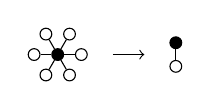
\begin{tikzpicture}
        \node [draw, fill, circle, inner sep=1.5pt] (A1) at (0, 0) {};
        \node [draw, circle, inner sep=1.5pt] (A2) at (0:0.3) {};
        \node [draw, circle, inner sep=1.5pt] (A3) at (60:0.3) {};
        \node [draw, circle, inner sep=1.5pt] (A4) at (120:0.3) {};
        \node [draw, circle, inner sep=1.5pt] (A5) at (180:0.3) {};
        \node [draw, circle, inner sep=1.5pt] (A6) at (240:0.3) {};
        \node [draw, circle, inner sep=1.5pt] (A7) at (300:0.3) {};

        \draw (A1) -- (A2);
        \draw (A1) -- (A3);
        \draw (A1) -- (A4);
        \draw (A1) -- (A5);
        \draw (A1) -- (A6);
        \draw (A1) -- (A7);

        \draw [->] (0.7, 0) -- (1.1, 0);

        \draw (1.5, 0) node [draw, fill, circle, inner sep=1.5pt] (B1) at ++ (90:0.15) {};
        \draw (1.5, 0) node [draw, circle, inner sep=1.5pt] (B2) at ++ (270:0.15) {};
        \draw (B1) -- (B2);
    \end{tikzpicture}\end{minipage}\hfill\begin{minipage}{3cm}
    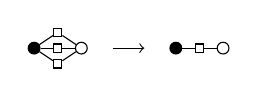
\begin{tikzpicture}
        \node [draw, fill, circle, inner sep=1.5pt] (A1) at (0, 0) {};
        \node [draw, inner sep=1.5pt] (A2) at (0.3, 0) {};
        \node [draw, inner sep=1.5pt] (A3) at (0.3, -0.2) {};
        \node [draw, inner sep=1.5pt] (A4) at (0.3, 0.2) {};
        \node [draw, circle, inner sep=1.5pt] (A5) at (0.6, 0) {};

        \draw (A1) -- (A2);
        \draw (A1) -- (A3);
        \draw (A1) -- (A4);
        \draw (A2) -- (A5);
        \draw (A3) -- (A5);
        \draw (A4) -- (A5);

        \draw [->] (1.0, 0) -- (1.4, 0);

        \node [draw, fill, circle, inner sep=1.5pt] (B1) at (1.8, 0) {};
        \node [draw, inner sep=1.5pt] (B2) at (2.1, 0) {};
        \node [draw, circle, inner sep=1.5pt] (B5) at (2.4, 0) {};

        \draw (B1) -- (B2);
        \draw (B2) -- (B5);
    \end{tikzpicture}\end{minipage}\hfill\,

    \bigskip

    \,\hfill\begin{minipage}{3cm}
    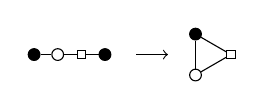
\begin{tikzpicture}
        \node [draw, fill, circle, inner sep=1.5pt] (A1) at (0, 0) {};
        \node [draw, circle, inner sep=1.5pt] (A2) at (0.3, 0) {};
        \node [draw, inner sep=1.5pt] (A3) at (0.6, 0) {};
        \node [draw, fill, circle, inner sep=1.5pt] (A4) at (0.9, 0) {};

        \draw (A1) -- (A2);
        \draw (A2) -- (A3);
        \draw (A3) -- (A4);

        \draw [->] (1.3, 0) -- (1.7, 0);

        \draw (2.2, 0) node [draw, fill, circle, inner sep=1.5pt] (B1) at ++ (120:0.3) {};
        \draw (2.2, 0) node [draw, circle, inner sep=1.5pt] (B2) at ++ (240:0.3) {};
        \draw (2.2, 0) node [draw, inner sep=1.5pt] (B3) at ++ (0:0.3) {};

        \draw (B1) -- (B2);
        \draw (B2) -- (B3);
        \draw (B3) -- (B1);
    \end{tikzpicture}\end{minipage}\hfill\begin{minipage}{3cm}
        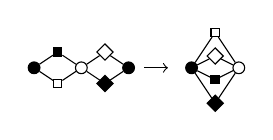
\begin{tikzpicture}
        \node [draw, fill, circle, inner sep=1.5pt] (A1) at (0, 0) {};
        \node [draw, inner sep=1.5pt] (A2) at (0.3, -0.2) {};
        \node [draw, fill, inner sep=1.5pt] (A3) at (0.3, 0.2) {};
        \node [draw, circle, inner sep=1.5pt] (A4) at (0.6, 0) {};
        \node [draw, diamond, fill, inner sep=1.5pt] (A5) at (0.9, -0.2) {};
        \node [draw, diamond, inner sep=1.5pt] (A6) at (0.9, 0.2) {};
        \node [draw, fill, circle, inner sep=1.5pt] (A7) at (1.2, 0) {};

        \draw (A1) -- (A2);
        \draw (A1) -- (A3);
        \draw (A2) -- (A4);
        \draw (A3) -- (A4);
        \draw (A4) -- (A5);
        \draw (A4) -- (A6);
        \draw (A5) -- (A7);
        \draw (A6) -- (A7);

        \draw [->] (1.4, 0) -- (1.7, 0);

        \node [draw, fill, circle, inner sep=1.5pt] (B1) at (2, 0) {};
        \node [draw, fill, inner sep=1.5pt] (B2) at (2.3, -0.15) {};
        \node [draw, diamond, inner sep=1.5pt] (B3) at (2.3, 0.15) {};
        \node [draw, diamond, fill, inner sep=1.5pt] (B4) at (2.3, -0.45) {};
        \node [draw, inner sep=1.5pt] (B5) at (2.3, 0.45) {};
        \node [draw, circle, inner sep=1.5pt] (B6) at (2.6, 0) {};

        \draw (B1) -- (B2);
        \draw (B1) -- (B3);
        \draw (B1) -- (B4);
        \draw (B1) -- (B5);
        \draw (B6) -- (B2);
        \draw (B6) -- (B3);
        \draw (B6) -- (B4);
        \draw (B6) -- (B5);
    \end{tikzpicture}\end{minipage}\hfill\,

    \caption{Counter-examples for various properties which are not invariants. The different shapes
        for vertices show a mapping, with vertices being mapped to vertices of the same shape. The
        top left example shows that degree is not preserved in a homomorphism; the top right that path
        counts are not preserved in a homomorphism; the bottom left that path counts of length three
        are not preserved in a locally injective homomorphism; and the bottom right that a locally
        injective homomorphism $i$ can give rise to a homomorphism $i^{2,2}$ which is not locally
        injective.} \label{figure:counterexamples}
\end{figure}

Constraint programming solvers can also exploit invariants that are based upon paths. This is done
by automatically adding \emph{implied} constraints to the problem that are implied by the original
model, but that will give stronger propagation.

\begin{proposition}[paths are preserved by subgraph isomorphisms]\label{proposition:distances}For
    the problem of finding a subgraph isomorphism $i$ from a graph $G$ to a graph $H$, the following
    constraints are implied for any pair of vertices $v, w \in \vertexset(G)$:
    \begin{enumerate}
        \item The distance between $v$ and $w$ is at most the distance between $i(v)$ and $i(w)$
            \cite{DBLP:conf/cp/AudemardLMGP14}.
        \item If there are at least $k$ simple
            paths of length exactly $\ell$ between $v$ and $w$, then there must be at least $k$
            simple paths of length exactly $\ell$ between $i(v)$ and $i(w)$
            \cite{DBLP:conf/cp/McCreeshP15}.
    \end{enumerate}
\end{proposition}

It is easy to verify that the first of these two properties is valid for \emph{any} homomorphism.
The second property does not hold for homomorphisms in general: for example, a pair of vertices
connected by three paths of length two may be mapped onto a pair of vertices connected by a single
path of length two (see \cref{figure:counterexamples}, top right). The second property also does not
hold in full generality for local injectivity, because, for example, a path of length three may be
mapped onto a triangle (\cref{figure:counterexamples}, bottom left): while standard injectivity
prevents any kind of merging, local injectivity only prevents two vertices from being merged if they
are both in the neighbourhood of the same vertex. However, a weaker result does hold:

\begin{proposition}[paths of length two are preserved by locally injective
    homomorphisms]\label{proposition:paths}For the problem of finding a locally injective graph
    homomorphism $i$ from a graph $G$ to a graph $H$, for any pair of vertices $v, w \in
    \vertexset(G)$, if there are at least $k$ simple paths of length exactly two between $v$ and
    $w$, then there must be at least $k$ simple paths of length exactly two between $i(v)$ and
    $i(w)$.
\end{proposition}

\begin{proof}Let $\{ x_1, \ldots, x_n \}$ be the intermediate vertices on the paths of length two
between $v$ and $w$. Observe that each $x_j$ is in the neighbourhood of $v$, and so must be mapped
    to different vertices. Thus each sequence $(i(v), i(x_j), i(w))$ gives a distinct simple path of
length two between $i(v)$ and $i(w)$.\end{proof}

Rather than using distance properties directly as \citet{DBLP:conf/cp/AudemardLMGP14} did,
\citet{DBLP:conf/cp/McCreeshP15} introduced the notion of \emph{supplemental} graphs, with the idea
that a constraint programming algorithm can search for a mapping which is simultaneously a subgraph
isomorphism between several different pairs of graphs. Let $G^d$ be the graph with the same set of
vertices as $G$, but with an edge between vertices $v$ and $w$ if the distance between $v$ and $w$
in $G$ is at most $d$.  Similarly, let $G^{n,\ell}$ be the graph with the same set of vertices as
$G$, but an edge between vertices $v$ and $w$ if there are at least $n$ simple paths of length
exactly $\ell$ between $v$ and $w$ in $G$. Following on from
\cref{proposition:distances,proposition:paths}, we generalise the result of
\citeauthor{DBLP:conf/cp/McCreeshP15} as follows.

\begin{corollary}Any homomorphism $i$ from $G$ to $H$ gives a homomorphism $i^d$ from $G^d$ to $H^d$
    defined by $i^d(v) = i(v)$, for all $d$. Furthermore, if $i$ is locally injective, then for all
    $n$, there is a homomorphism $i^{n,2}$ from $G^{n,2}$ to
    $H^{n,2}$ defined by $i^{n,2}(v) = i(v)$.\label{corollary:lishapes}
\end{corollary}

Note carefully that $i^{n,2}$ is \emph{not} necessarily locally injective, even if $i$ is; we
illustrate a counter-example in \cref{figure:counterexamples} (bottom right). This is in contrast to
subgraph isomorphism, where $i^{n,\ell}$ is a subgraph isomorphism for all $\ell$
\cite{DBLP:conf/cp/McCreeshP15}.

We now discuss the main new technique of this paper. Observe
that so far, we have not seen any unary constraints which are valid for the general homomorphism
problem. All existing constraint programming approaches for the subgraph isomorphism problem begin
by branching on the variable which has the smallest domain---typically this will be a domain for a
vertex of high degree, or which has many high degree neighbours. Furthermore, once one such
guessed assignment has been made, adjacency propagation means many other domains will be
substantially reduced in size, making subsequent branching choices simpler.  However, for
homomorphism problems, if we cannot find any implied unary constraints then every domain will
initially be of the same size, which will make it much harder for a solver to know where to start.
This motivates the following.

\begin{proposition}[Cliques are preserved]\label{proposition:clique}
    Let $i$ be a homomorphism from $G$ to $H$ where $H$ does
    not contain any loops. Let $S\subseteq V$ be such that $G[S]$ is a $k$-vertex clique. Then
    $H[i(S)]$ is also a $k$-vertex clique.
\end{proposition}

\begin{proof}
    Let $j$ and $k$ be two distinct vertices of the clique in $G$. By definition of a homomorphism,
    $i(j)$ and $i(k)$ must be adjacent. And, because $H$ has no loops, $i(j) \ne i(k)$.
\end{proof}

\begin{corollary}\Cref{proposition:clique} holds for locally injective graph homomorphisms and for
    subgraph isomorphisms even if loops are present in the second graph.
\end{corollary}

Next we will discuss how this is useful in practice.

\section{Design and Implementation}

Having determined which commonly-used subgraph isomorphism invariants do and do not hold for other
forms of homomorphism, and having discovered a new clique-based invariant, we will now look at how
these invariants may be used in practice. Our starting point is the Glasgow Subgraph Solver
\cite{DBLP:conf/gg/McCreeshP020}, due to it being the current strongest solver for
subgraph isomorphism. Adapting the solver to handle locally injective and general homomorphism
problems required the following straightforward changes.

\paragraph{Injectivity constraints.} For subgraph isomorphism, injectivity is handled by a
combination of binary constraints and a specialised bit-parallel all-different propagator
\cite{DBLP:conf/cp/McCreeshP15}. This was disabled entirely for homomorphism problems, and for local
injectivity only binary constraints were used.

\paragraph{Path-based filtering.} For subgraph isomorphism, the Glasgow Subgraph Solver
searches for a mapping which is simultaneously a subgraph isomorphisms between $(G, H)$ and each
$(G^{n,2}, G^{n,2})$ for each $n$ from $1$ to $4$, and optionally also between $(G^3, H^3)$. For
homomorphisms, we use $(G^2, H^2)$, whilst for locally injective homomorphisms we use $(G^{n,2},
G^{n,2})$ for each $n$ from $1$ to $4$.

\paragraph{Degree-based filtering.} This was disabled for homomorphisms and left enabled for locally
injective homomorphisms, as per \cref{proposition:degreends}. For subgraph isomorphism, the Glasgow
Subgraph Solver uses degree and neighbourhood degree sequences not just on the original graphs, but
also on each $(G^{n,\ell}, H^{n,\ell})$ graph pair. This is \emph{not} possible for locally
injective homomorphisms, due to the counter-example following \cref{corollary:lishapes}.

\paragraph{Search order heuristics.} The solver's default search order heuristics are based upon
three principles: that it is good to branch on variables with few remaining values in a domain, that
it is good to branch on variables corresponding to high-degree vertices, and that it is good to try
mapping to vertices of high degree
\cite{DBLP:journals/jair/McCreeshPST18,DBLP:conf/cpaior/ArchibaldDHMP019}. These principles do not
appear to be specific to subgraph isomorphism, and so we do not alter the search order heuristics.

\paragraph{Loops.} For the homomorphism decision problem, we modified the solver so that if the
codomain graph contains a loop, we immediately return a satisfying assignment mapping every vertex
to one of these loops.

\subsection{Clique Filtering}

Implementing clique constraints required substantially more work. The Glasgow Subgraph Solver
contains a maximum clique implementation, which is based upon a variation of
\citet{DBLP:conf/walcom/TomitaSHTW10}'s MCS algorithm which
\citet{DBLP:journals/algorithms/Prosser12} calls ``MCSa1'', with bit-parallelism
\cite{DBLP:journals/ol/SegundoMRH13} and an altered
branching scheme for faster optimality proofs \cite{DBLP:conf/cp/McCreeshP14}. The implementation
also makes use of a shortcut due to \citet{DBLP:journals/jco/BatsynGMP14}, which allows certain
cliques to be detected without branching---this turns out to be particularly useful in this setting,
making many of the clique instances generated solvable without branching.
Initially we used this solver to perform domain filtering as a preprocessing step. Preliminary
experiments showed that a na{\"\i}ve approach, which calculates the maximum clique size for
the neighbourhood of each domain vertex and each codomain vertex, would add as much as three minutes
of preprocessing time to some problem instances which could otherwise be solved in a few seconds. We
therefore invested more engineering effort, as follows.

Assuming a problem instance is not detected as obviously unsatisfiable, we calculate the maximum
clique size for the neighbourhood of every domain vertex in turn. However, having found a maximum
clique with $k$ vertices in the neighbourhood of a vertex $p$, we remember for every other vertex in
this maximum clique that its neighbourhood maximum clique size is at least $k$. This can be used to
accelerate subsequent clique solver calls, by starting the branch and bound algorithm with an
initial incumbent size of $k$ rather than zero.

We then move on to the codomain vertices, using a similar caching routine. Rather than calculating a
clique size for every single codomain vertex, we only calculate a value for codomain vertices which are
present in at least one variable's domain, after other unary constraints have been applied.
Additionally, we do not require the maximum clique solver to run to completion and guarantee that it
has found a maximum clique. Instead, we allow it to stop as soon as it has found a clique with as
many vertices as the largest domain clique. This is useful because it may be very hard to decide
whether a particular codomain vertex has neighbourhood clique size of, say, 15 or 16, but if the
largest domain vertex has a neighbourhood clique size of only 5 then this is irrelevant.

\subsection{Proof Logging}

Given the complexity of modern solvers, a critical question is how we can be sure that they are
producing correct answers. The Glasgow Subgraph Solver's subgraph isomorphism and clique algorithms
are both \emph{certifying} \cite{DBLP:journals/csr/McConnellMNS11}: that is, they can output a
mathematical proof that they have reached a correct answer by sound reasoning, and this proof log
can be verified by the VeriPB proof checking tool
\cite{DBLP:conf/cp/GochtMMNPT20,DBLP:conf/ijcai/GochtMN20}. We therefore extended the solver's
existing proof logging support to cover our additions. For the changes not involving clique-finding,
this was entirely routine---although proof logging did catch an implementation bug where we were
incorrectly applying degree-based filtering on the $G^{2,n}$ graphs for locally injective
homomorphisms, in violation of the counter-example to \cref{corollary:lishapes}. For clique-based
filtering, the process involved substantially more technical work. Briefly, for a given domain
vertex $v$ that cannot be mapped to a codomain vertex $w$, it is possible to instruct the proof
verifier to derive a set of conditional clique constraints saying that ``either $v$ cannot be mapped
to $w$, or the following clique-like problem must be satisfiable'' by following steps similar to the
maximum common subgraph to clique reduction presented by \citet{DBLP:conf/cp/GochtMMNPT20}, and then
to reuse clique proof-logging techniques to show that this clique-like problem is unsatisfiable.  We
were able to produce and verify proofs of correctness for medium-sized instances, giving us
confidence in our implementation.

This situation is not entirely ideal. The proofs produced this way are inherently dependent upon a
\emph{particular} choice of domain and codomain vertices. Thus, when proof logging, we must solve
restricted clique problems for each assignment that is to be filtered using a clique rule, rather
than for each clique found; this is potentially a linear factor blowup.  This seems wasteful, since
for any given codomain vertex these proofs are effectively the same up to substitution of variable
names. It would therefore seem desirable to extend the proof system with a substitution rule which
would allow such proofs to be recycled to avoid duplication.

\section{Experiments}

\begin{figure*}[p]
    \,\hfill\begin{tabular}{c@{}c@{}c@{}}
    \includegraphics{gen-graph-cumulatives.pdf}
        &
    \includegraphics{gen-graph-cumulatives-differences.pdf}
        &
    \includegraphics{gen-graph-cumulatives-aggregate.pdf}
        \\[5mm]
    \includegraphics{gen-graph-cumulatives-hom.pdf}
        &
    \includegraphics{gen-graph-cumulatives-local.pdf}
        &
    \includegraphics{gen-graph-cumulatives-si.pdf}
    \end{tabular}\hfill\,

    \caption{On the top left, the cumulative number of instances solved over time for the three
    problem variants, with and without clique filtering, and with and without distance filtering for
    the homomorphism problem; for comparison, results for subgraph isomoprhism using the PathLAD,
    RI, and VF2 solvers are also shown. The remaining plots re-display this data, as follows. The
    three plots on the bottom row zoom in on the cumulative number of instances solved, for the
    homomorphism problem on the left, the locally injective homomorphism problem in the centre, and
    the subgraph isomorphism problem on the right. The top centre plot shows the additional number
    of instances solved at any given time when using the new forms of filtering for all problem
    variants, and the top right plot shows the aggregate speedups from each form of
    filtering.}\label{figure:plots}
\end{figure*}
\begin{figure*}[p]
    \,\hfill\begin{tabular}{c@{\hspace{4mm}}c@{\hspace{4mm}}c@{\hspace{4mm}}c@{\hspace{4mm}}}
        \includegraphics{gen-graph-scatter-hom-c.pdf}
        &
        \includegraphics{gen-graph-scatter-hom-cd.pdf}
        &
        \includegraphics{gen-graph-scatter-local.pdf}
        &
        \includegraphics{gen-graph-scatter-si.pdf}
    \end{tabular}\hfill\,

    \caption{Looking at the effects of additional filtering on an instance by instance basis, for
    homomorphism with just clique filtering and with both clique and distance filtering, and for the
    other two variants with clique filtering. Each point represents one instance, the vertical axis
    is the runtime with filtering in ms, and the horizontal axis is the runtime without filtering in
    ms (and so points below the diagonal are speedups). Points on the outer axes are timeouts. The
    different point styles show the different families of instance from the benchmark set, and
    illustrate that in each the filtering is broadly useful rather than being specific to a single
    kind of application.}\label{figure:scatters}
\end{figure*}

We now evaluate this approach empirically. Our experiments are performed on a cluster of machines
with dual Intel Xeon E5-2697A v4 CPUs with 512GBytes of RAM, running Ubuntu 18.04, and using a
timeout of one hour; we do not enable proof logging for these benchmarks since proof logging
introduces large slowdowns due to I/O costs \cite{DBLP:conf/cp/GochtMMNPT20}. Because injectivity
relaxations have received less attention until now, for all three problem variants we will use a
suite of 14,621 benchmark instances designed for the subgraph isomorphism problem
\cite{DBLP:conf/lion/KotthoffMS16}. Note that 8,904 of these instances contain at least one loop in
the codomain graph, and so are trivial for the homomorphism problem---we still include these to
avoid using different y-axes on different plots.

In the top left plot of \cref{figure:plots} we show the cumulative number of instances solved over
time, for each of the three problem variants, using the Glasgow Subgraph Solver with and without our
clique-filtering added. For the homomorphism problem, we also compare with distance filtering
enabled or disabled. For subgraph isomorphism, we further compare against the PathLAD
\cite{DBLP:conf/lion/KotthoffMS16}, VF2 \cite{DBLP:journals/pami/CordellaFSV04} and RI
\cite{DBLP:journals/bmcbi/BonniciGPSF13} solvers. To make the details of this plot readable, the
second row of \cref{figure:plots} zooms in on the results for each
problem variant in turn. We see that for the homomorphism problem, using either clique or
distance filtering gives a clear improvement to performance, and using both together is better
still. For both injective problems, clique filtering gives a more moderate improvement.

To quantify these gains, the top centre plot of \cref{figure:plots} shows the
additional number of instances solved at any given time (that is, the vertical distance between
two cumulative plots) when enabling additional filtering. We see that for subgraph isomorphism, at
the one hour timeout we solve 22 additional instances using clique filtering; for locally injective
homomorphisms, 21 additional instances; and for homomorphisms, 114, 146 or 193 additional instances
using just distance filtering, just clique filtering, or both. Or, at the best choices of timeouts,
we solve 53 additional subgraph isomorphism instances; 64 additional locally injective instances;
and 243, 383, and 424 additional homomorphism instances.

Alternatively, we can measure the horizontal distance between plots for a given choice of timeout
$t$ as follows. Let $t'$ be the last time no greater than $t$ where the slower algorithm solved an
instance, and let $u$ be the lowest amount of time needed for the faster algorithm to solve the same
number of instances.  The \emph{aggregate speedup}, which we plot in the top right of
\cref{figure:plots}, is the ratio of $t'$ to $u$ or $u$ to $t'$ as appropriate. At the one hour
timeout, we see aggregate speedups of 2.2 for locally injective homomorphisms, 3.2 for subgraph
isomorphism, and 47.5, 131.7, and 803.5 for homomorphisms.

The crossover point, where clique filtering begins to pay off, is at around the 100ms mark without
injectivity, and at around one second for the injective problems. This does not show how much time
was spent in clique-finding, but rather how long it takes for an algorithm with increased
filtering to catch up from a slower start. In fact, for domain graphs, no maximum clique call took
even one millisecond to complete (and none required more than two hundred recursive calls from the
clique solver), and more time was spent setting up the data structures to represent the
neighbourhood graphs than on the actual solving. For codomain graphs, 20,838,008 of the clique
problems we solved took under a millisecond, and the remaining 279 calls took between one and four
milliseconds, with no instance requiring more than a thousand recursive calls.  Although it may seem
counter-intuitive to try to speed up the solving of a hard problem by first solving many other hard
problems, these values demonstrate that clique-solving on these smaller graphs is \emph{much} easier
in practice than solving the larger problem, and so is worthwhile.

Finally, \cref{figure:scatters} plots instance-by-instance comparisons of the runtimes. The
point styles in these plots show different families of benchmark instance, and demonstrate
that the benefits of filtering are not restricted to one application. They also show that clique
filtering very rarely makes performance a lot worse, but often makes it a lot better.

\section{Conclusion}

Our results have shown that constraint programming approaches are viable for a wider range of subgraph
mapping finding problems than had previously been considered, and will increase the versatility of
subgraph solvers for application users going forwards. We saw that using clique-finding as a
filtering step could give moderate to very large speedups for different problem variants---although
only through careful engineering choices, to mitigate the potential cost of solving \NP-hard
problems. We would be interested to see if filtering based upon other hard problems could give
similar benefits---for example, homomorphisms also interact in potentially helpful ways with various
colouring properties.

\section*{Acknowledgements}

This work was supported by the Engineering and Physical Sciences Research Council [grant number
EP/P026842/1].

\bibliographystyle{named}
\bibliography{paper}

\end{document}

% vim: set tw=100 spell spelllang=en : %
